Die Roboterzelle ist im Rahmen dieses Testszenarios als isolierter Arbeitsraum
mit mehreren Hindernissen, Begrenzungen und 3 semantischen Stationen aufgebaut.
Die vom Roboter zu bewältigenden Aufgaben beschränken sich dabei auf ein
Pick-and-Place-Szenario von Zylinderköpfen, dargestellt in
Abbildung~\ref{figure:arbeitsraum}.

\begin{figure}[H]
  \centering
  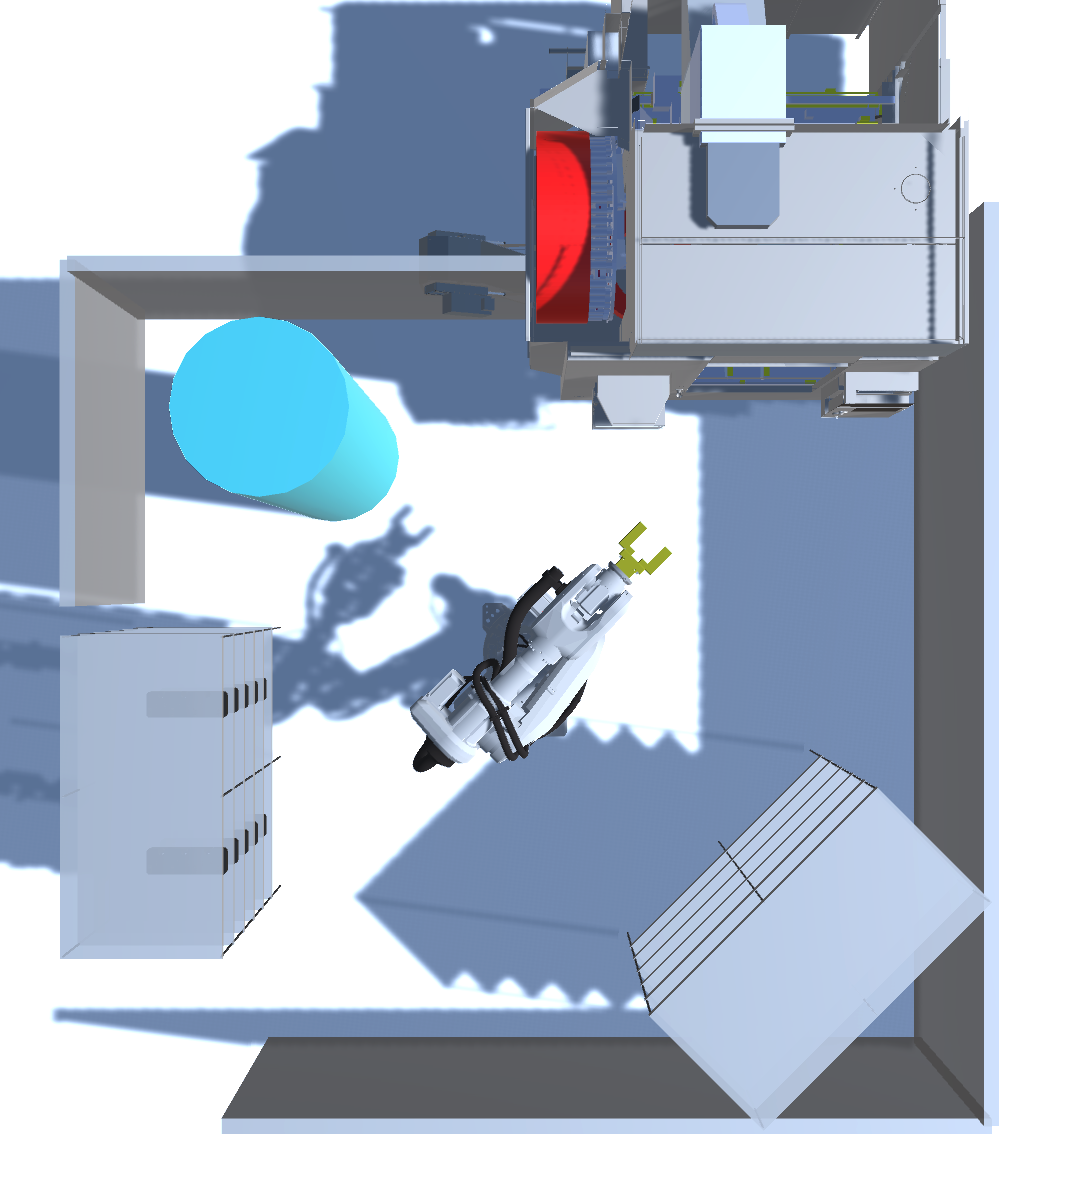
\includegraphics[width=10cm]{Figures/Roboterzelle.png}
  \caption{Arbeitsraum-Layout des Roboters in der Draufsicht mit Roboter in
  Home-Position}
  \label{figure:arbeitsraum}
\end{figure}

Das hierfür erstellte Layout sieht den Roboter in Zentrum des Arbeitsraumes auf
dem Boden stehend vor. Hindernisse, Begrenzungen und Stationen sind kreisförmig
um den Roboter angeordnet. In Abbildung
\ref{figure:arbeitsraum}
blau markiert, befindet sich eine Säule als künstliches Hindernis.
Links und rechts unten vom Mittelpunkt der Zelle aus befinden sich
zwei Regale als Teilelager. Oben befindet sich eine 5-Achs-Fräsmaschine mit
einer offenen Teileablage durch Entfernung der Schutztür zu
Vereinfachungszwecken dieses Szenarios. Der Arbeitsraum ist begrenzt durch
halbdurchsichtige Wände. Der Prozessablauf sieht vor, dass der Roboter
Zylinderköpfe aus dem linken Regal aufnimmt, diese in der Maschine ablegt, in
einer Warteposition auf die Beendigung der Bearbeitung wartet und anschließend
das bearbeitete Teil aufnimmt, um es im rechten Regal abzulegen. Ein
beispielhafter Bearbeitungsprozess mit der 5-Achs-Fräsmaschine ist
hier das Bohren und Schneiden von Gewinden
in die Zylinderköpfe.

Der Aufbau und die Anordnung des Arbeitsraums ergibt sich aus den funktionalen
Anforderungen, die das Framework abdecken soll. Durch den relativ begrenzten
Raum müssen Bewegungspfade des Roboters an Hindernissen,
beispielsweise der Säule, vorbei
geplant werden und etwaige durch den Roboter gegriffene Werkstücke
mitberechnet werden. Weiterführend verringern die Regale den Bewegungsraum für
den Roboter zur Umorientierung vor sowie nach dem Aufnehmen und
Ablegen der Teile,
was zu einer erhöhten Wahrscheinlichkeit von Singularitäten führt. Die drei
semantischen Stationen sorgen dafür, dass sich hier Fehler im Prozessablauf
abbilden lassen. Die Achsgeschwindigkeiten lassen sich in diesem Szenario
ebenfalls beliebig variieren. Somit lassen sich alle funktionalen Anforderungen
des Frameworks innerhalb dieses vereinfachten Szenarios abbilden.

\subsubsection{Zylinderköpfe als Werkstücke}
Als Werkstücke werden hier Zylinderköpfe für V6-Motoren gewählt. Das Werkstück
bringt ein mit den Spezifikationen des ABB IRB 6700 übereinstimmendes Gewicht
mit und ist an den Seitenflächen durch einen Parallelgreifer gut greifbar. Die
Abmaße, des Zylinderkopfes sind Abbildung \ref{figure:cylinderhead}
zu entnehmen.

\begin{figure}[H]
  \centering
  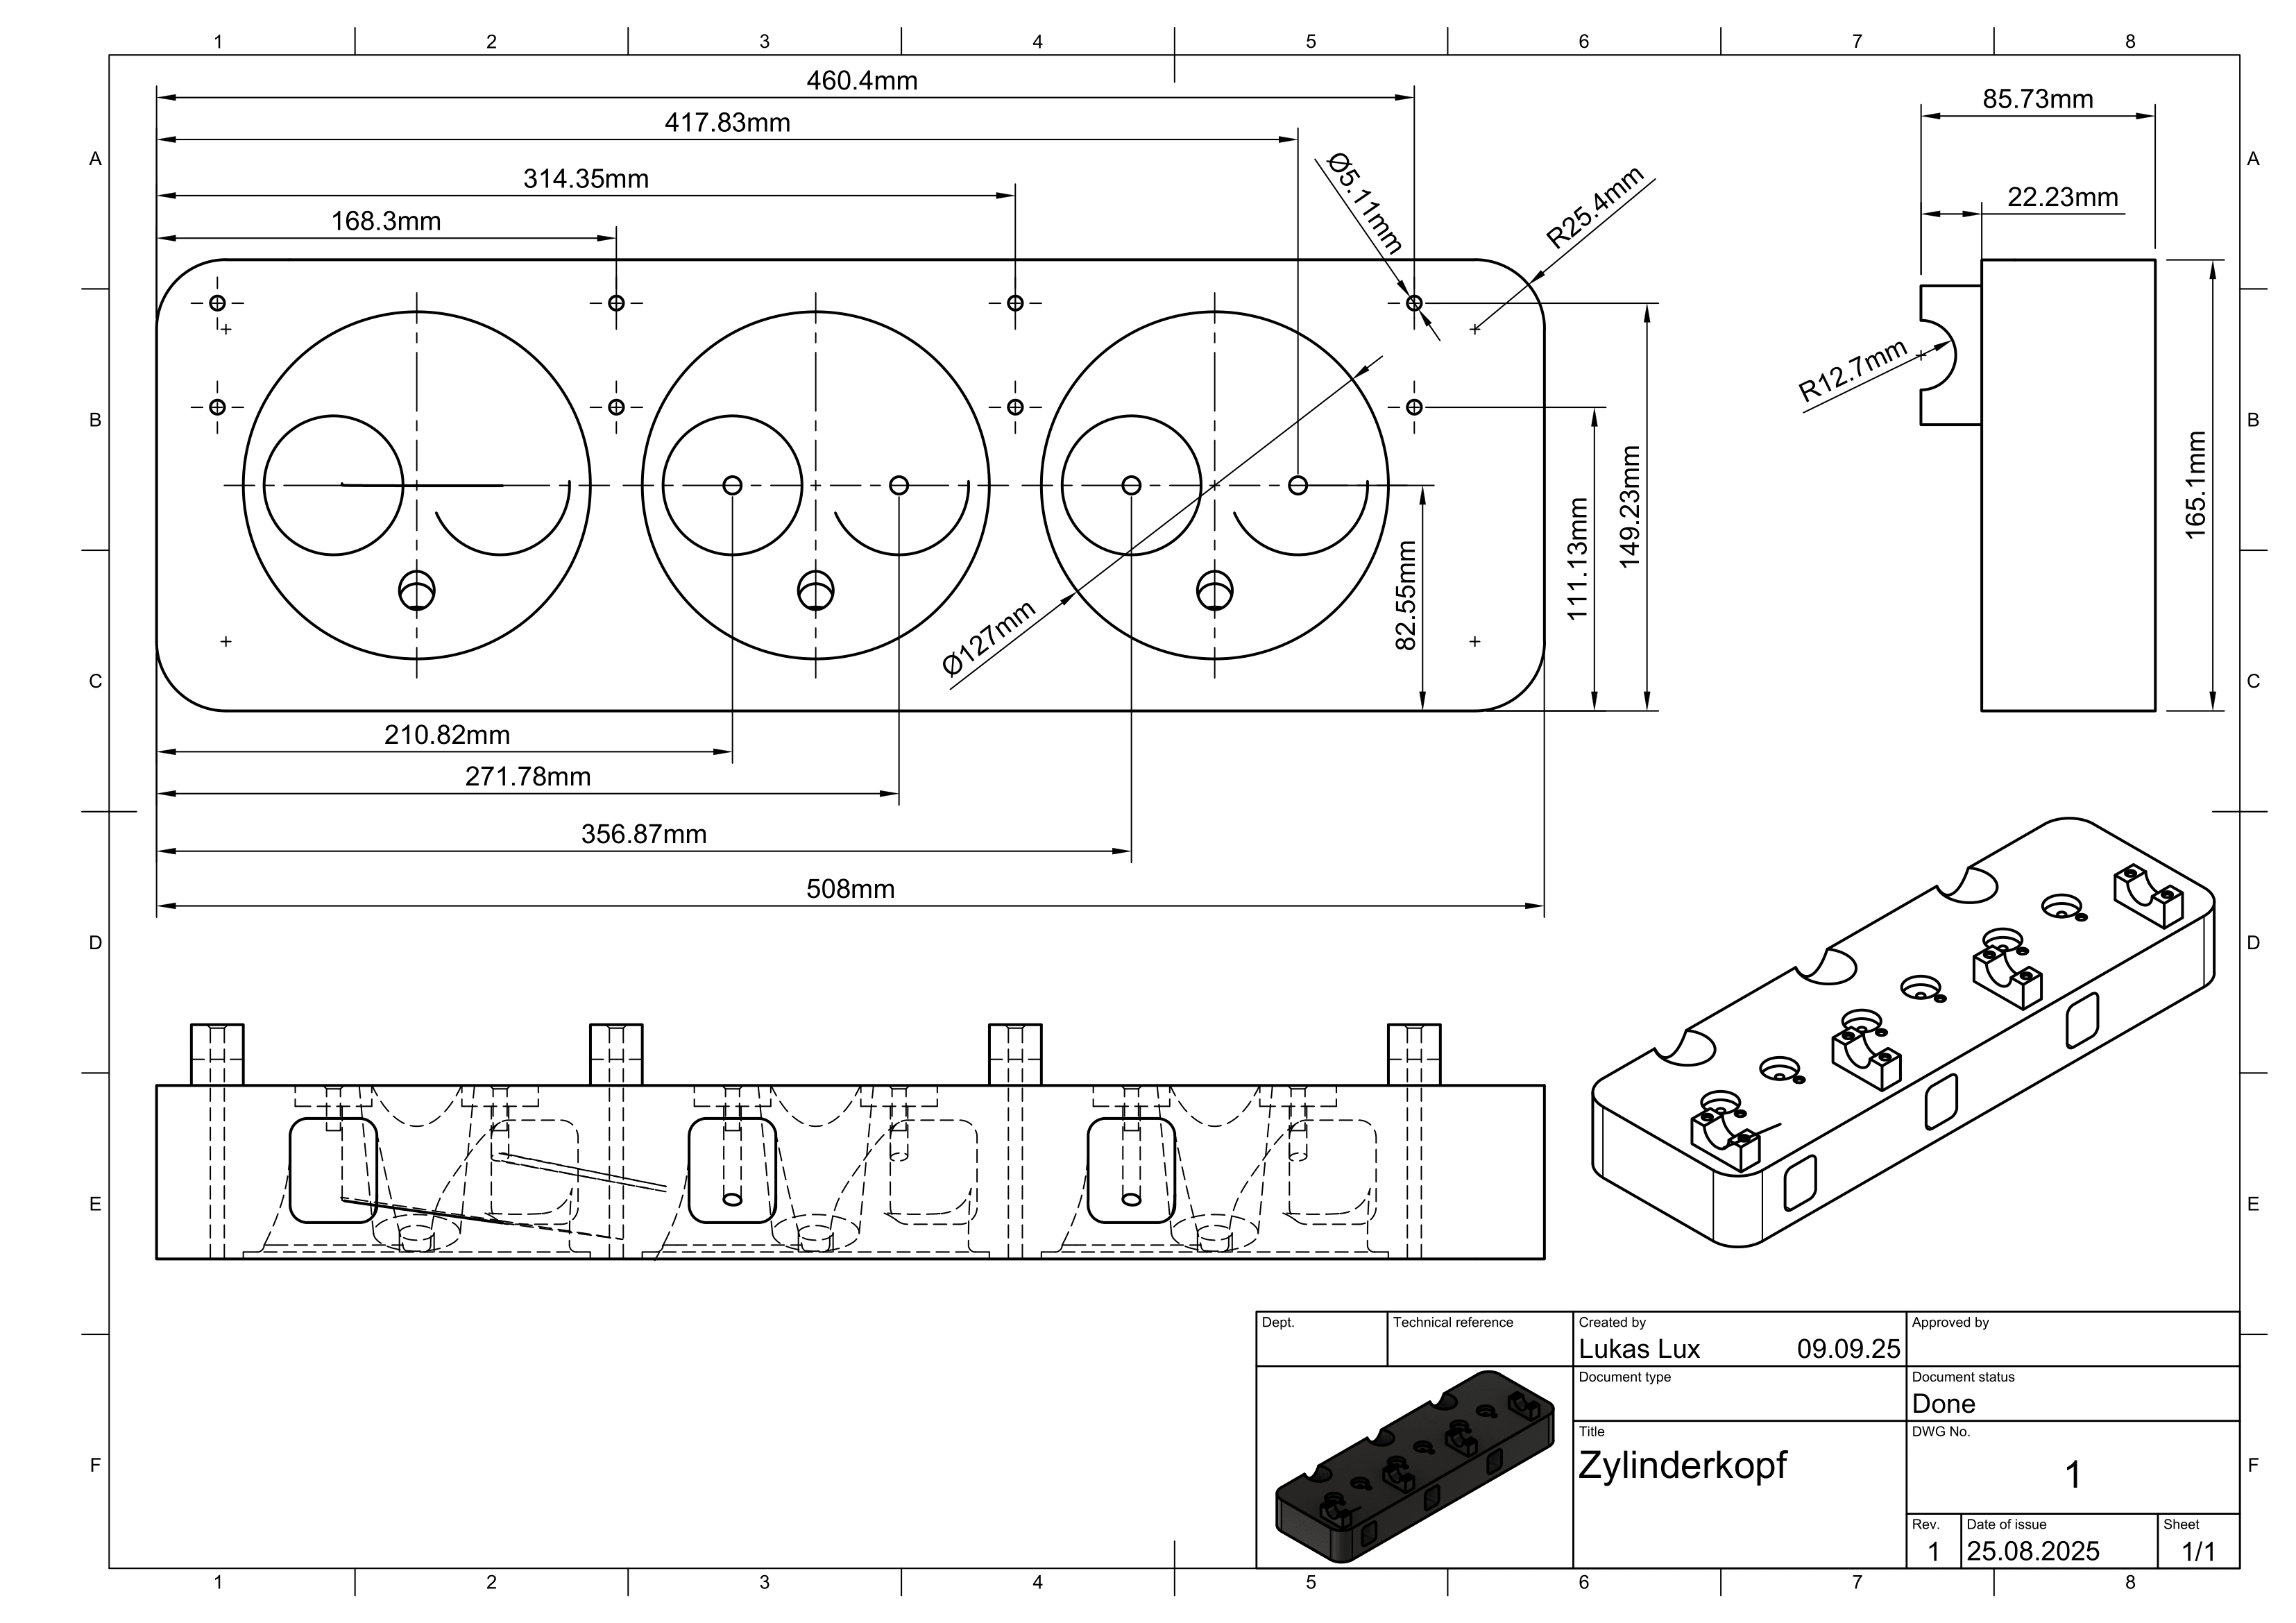
\includegraphics[width=\linewidth]{Figures/CyclinderHead-1.png}
  \caption{Technische Zeichnung des verwendeten Zylinderkopfes, dargestellt
  mithilfe von Autodesk Fusion 360}
  \label{figure:cylinderhead}
\end{figure}

\subsubsection{Greiferauslegung}

Um das Werkstück sicher handhaben zu können, wird zusätzlich zum Roboter
ein End-Effektor benötigt, welcher das Werkstück sicher durch den Arbeitsraum
bewegen kann. Hierzu wird ein Parallelgreifer verwendet, welcher speziell zu
Handhabung des Zylinderkopfes ausgelegt wurde.
Da das Anforderungsprofil von End-Effektoren kaum normierbar und
werkstückabhängig ist, ist die Auslegung eines
spezifischen Greifers für die Handhabung individueller Werkstücke gängige
Praxis.\vglcite[91]{hesse2011}

Mithilfe eines Online-Konfigurationstools der Firma
SCHUNK\vglcite{schunk2025} ist es möglich, einen parametrisierten
Greifer auszulegen und als
3D-CAD-Modelle in verschiedenen Formaten herunterzuladen. Hier wurde
aufgrund der
Werkstückdimensionen ein Parallelgreifer der Baureihe PGN-Plus-P gewählt und die
Form der Greifbacken dem Werkstück entsprechend angepasst (siehe
Abbildung~\ref{figure:schunkGripper}).

\begin{figure}[H]
  \centering
  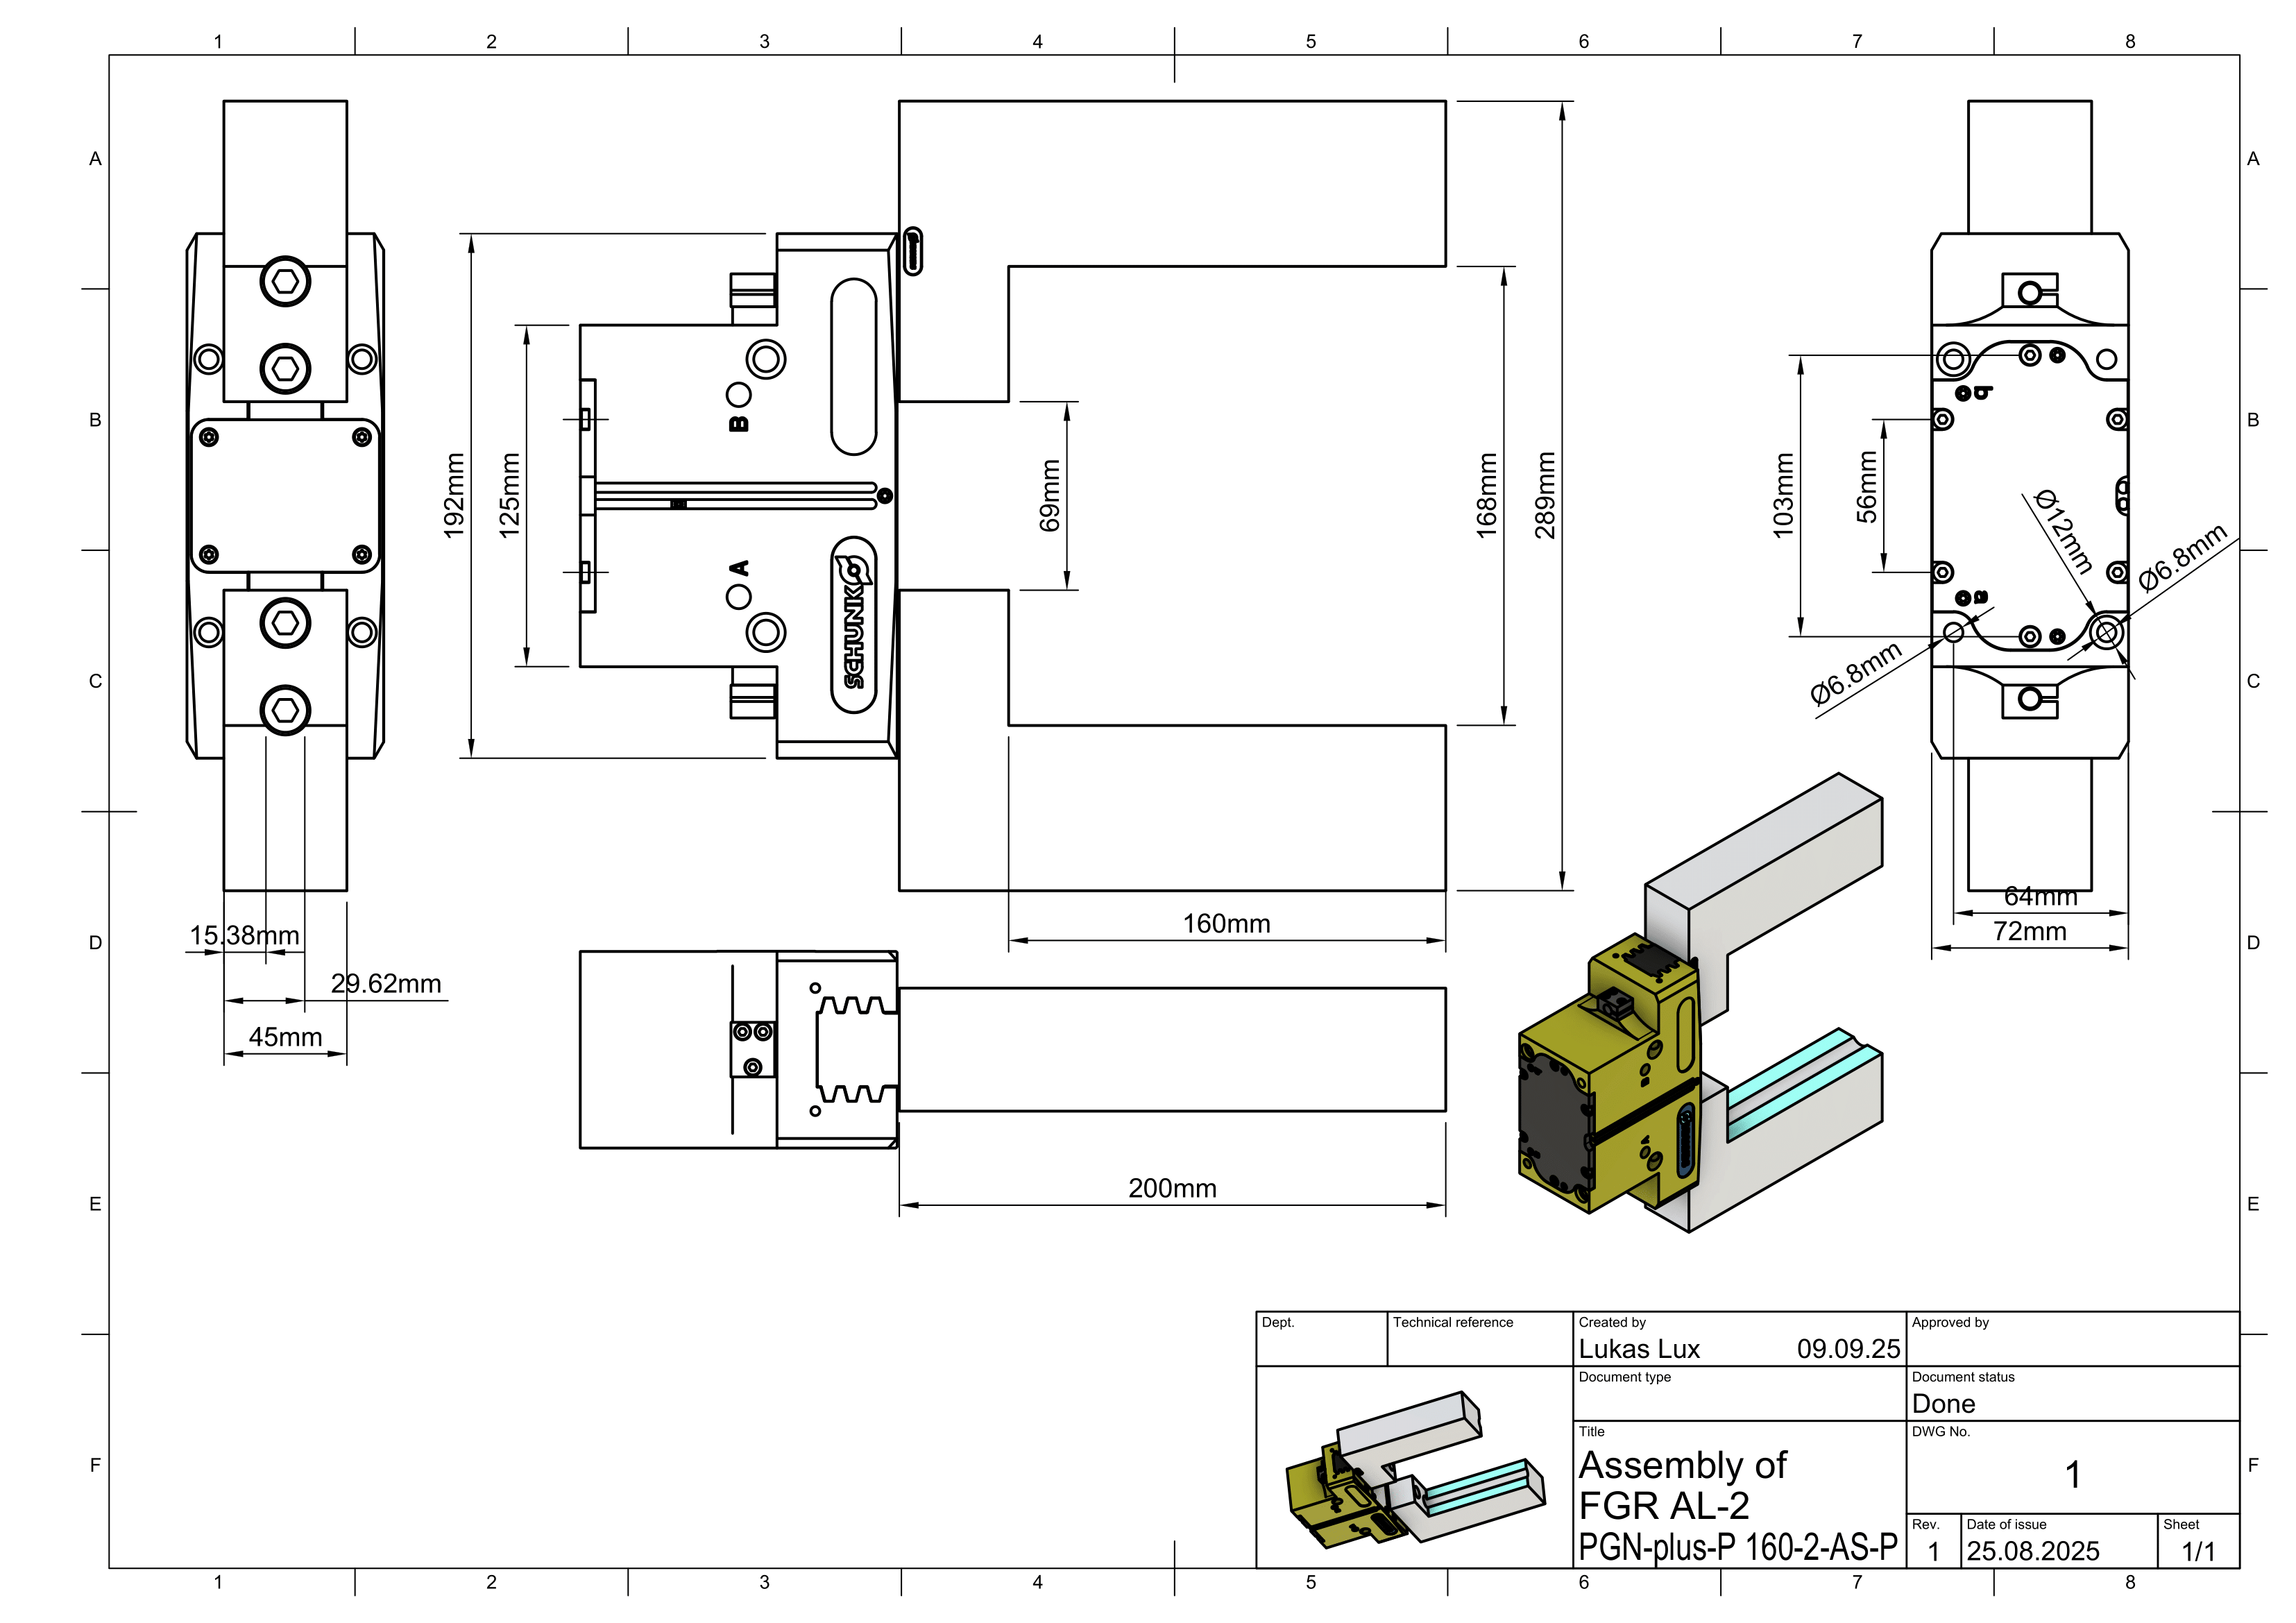
\includegraphics[width=\linewidth]{Figures/SchunkGreifer-1.png}
  \caption{Technische Zeichnung des ausgelegten Parallelgreifers, dargestellt
  mithilfe von Autodesk Fusion 360}
  \label{figure:schunkGripper}
\end{figure}

\subsection{Flange als Visualisierungstool}
Im Rahmen dieses Frameworks wird das Unity-Package \textit{Flange} genutzt.
Implementiert durch GitHub-User \textit{Preliy} und frei verfügbar im Rahmen
einer BSD 3-Clause Lizenz, bietet ein spezialisiertes Framework für die
Robotersteuerung in Unity mit modularer Architektur, die Gelenksteuerung,
Kinematik, Koordinatentransformationen und Echtzeitüberwachung als separate
Komponenten organisiert. Das System unterstützt sowohl direkte
Gelenkmanipulation auf niedriger Ebene als auch kartesische Steuerung auf
höherer Abstraktionsebene, wodurch es für verschiedene Roboteranwendungen
einsetzbar ist.\vglcite{preliyflange2024} Im Kontext dieser Entwicklungsarbeit
wird Flange zur Implementierung und Visualisierung der
Denavit-Hartenberg-Parameter und damit einhergehender Achstransformationen
eingesetzt. Die Notation nach Denavit-Hartenberg ermöglicht als
fundamentales Werkzeug der Robotik eine
systematische Beschreibung der Geometrie serieller Robotermechanismen
und somit die Anwendung etablierter algorithmischer Verfahren für kinematische
Berechnungen, Berechnung von Jacobi-Matrizen sowie
Bewegungsplanung.\vglcite[590]{corke2007}

Flange ermöglicht eine direkte Konfiguration des Roboters über \textit{Frame}
und \textit{JointTransformation} Scripts. Ein Frame definiert dabei die
Denavit-Hartenberg-Parameter für einen Teil der kinematischen Kette, eine
JointTransformation die Parameter des Gelenks, also möglicher
maximaler Ausschlag
in positive und negative Achsrotationsrichtung sowie maximale Geschwindigkeit
und Beschleunigung. Diese Funktion werden im Rahmen dieser Implementierung
genutzt, um den zu simulierenden Roboter theoretisch nachvollziehbar im Raum
bewegen zu können.

\subsection{Modellierung in Unity}
Der Arbeitsraum wurde der vorangegangenen Darstellung entsprechend in Unity
modelliert. Dabei wurden die von Unity standardmäßig gewählten Einstellungen
verwendet, sowohl bei der Modellierung als auch im Kontext der
Physik-Engine. Jegliche Hindernisse wurden dabei mit Collidern versehen und dem
Tag \texttt{Obstacle} und respektive \texttt{Machine} für die Maschine, um diese
bei der späteren Auswertung als Hindernisse kenntlich zu machen. Weiterführend
wurden den einzelnen Stationen (linkes und rechtes Regal, Maschine) das Script
\texttt{Station.cs} angehängt und dort im Sinne des bereits beschriebenen
Arbeitsablaufs ein steigender Index zugewiesen. Analog dazu wird allen
Zylinderkopf-Objekten das Script \texttt{Part.cs} zugewiesen, welche diese als
Werkstücke identifiziert und mit dem durch Drag-and-Drop im Unity Inspector die
Reihenfolge der einzelnen Stationen definiert wird, welche das Teil durchlaufen
muss.

Alle Monitore wurden in einer einheitlichen Unity-Testumgebung ausgeführt.
Die Simulationen basieren auf einem Abbild des Roboters, der
kontinuierlich seine Gelenkwinkel und Zustände an die Monitore übermittelt.
Die erkannten Ereignisse werden unmittelbar protokolliert und in eine
JSON-Logdatei geschrieben. Auf diese Weise sind die Ergebnisse der
verschiedenen Monitore konsistent dokumentiert und in
Kapitel~\ref{cap:Ergebnisse} direkt vergleichbar.
